% Options for packages loaded elsewhere
\PassOptionsToPackage{unicode}{hyperref}
\PassOptionsToPackage{hyphens}{url}
%
\documentclass[
  english,
]{article}
\usepackage{lmodern}
\usepackage{amssymb,amsmath}
\usepackage{ifxetex,ifluatex}
\ifnum 0\ifxetex 1\fi\ifluatex 1\fi=0 % if pdftex
  \usepackage[T1]{fontenc}
  \usepackage[utf8]{inputenc}
  \usepackage{textcomp} % provide euro and other symbols
\else % if luatex or xetex
  \usepackage{unicode-math}
  \defaultfontfeatures{Scale=MatchLowercase}
  \defaultfontfeatures[\rmfamily]{Ligatures=TeX,Scale=1}
\fi
% Use upquote if available, for straight quotes in verbatim environments
\IfFileExists{upquote.sty}{\usepackage{upquote}}{}
\IfFileExists{microtype.sty}{% use microtype if available
  \usepackage[]{microtype}
  \UseMicrotypeSet[protrusion]{basicmath} % disable protrusion for tt fonts
}{}
\makeatletter
\@ifundefined{KOMAClassName}{% if non-KOMA class
  \IfFileExists{parskip.sty}{%
    \usepackage{parskip}
  }{% else
    \setlength{\parindent}{0pt}
    \setlength{\parskip}{6pt plus 2pt minus 1pt}}
}{% if KOMA class
  \KOMAoptions{parskip=half}}
\makeatother
\usepackage{xcolor}
\IfFileExists{xurl.sty}{\usepackage{xurl}}{} % add URL line breaks if available
\IfFileExists{bookmark.sty}{\usepackage{bookmark}}{\usepackage{hyperref}}
\hypersetup{
  pdftitle={PEC2 Análisis de Datos Ómicos},
  pdfauthor={Rita Ortega Vallbona},
  hidelinks,
  pdfcreator={LaTeX via pandoc}}
\urlstyle{same} % disable monospaced font for URLs
\usepackage[margin=1in]{geometry}
\usepackage{color}
\usepackage{fancyvrb}
\newcommand{\VerbBar}{|}
\newcommand{\VERB}{\Verb[commandchars=\\\{\}]}
\DefineVerbatimEnvironment{Highlighting}{Verbatim}{commandchars=\\\{\}}
% Add ',fontsize=\small' for more characters per line
\usepackage{framed}
\definecolor{shadecolor}{RGB}{248,248,248}
\newenvironment{Shaded}{\begin{snugshade}}{\end{snugshade}}
\newcommand{\AlertTok}[1]{\textcolor[rgb]{0.94,0.16,0.16}{#1}}
\newcommand{\AnnotationTok}[1]{\textcolor[rgb]{0.56,0.35,0.01}{\textbf{\textit{#1}}}}
\newcommand{\AttributeTok}[1]{\textcolor[rgb]{0.77,0.63,0.00}{#1}}
\newcommand{\BaseNTok}[1]{\textcolor[rgb]{0.00,0.00,0.81}{#1}}
\newcommand{\BuiltInTok}[1]{#1}
\newcommand{\CharTok}[1]{\textcolor[rgb]{0.31,0.60,0.02}{#1}}
\newcommand{\CommentTok}[1]{\textcolor[rgb]{0.56,0.35,0.01}{\textit{#1}}}
\newcommand{\CommentVarTok}[1]{\textcolor[rgb]{0.56,0.35,0.01}{\textbf{\textit{#1}}}}
\newcommand{\ConstantTok}[1]{\textcolor[rgb]{0.00,0.00,0.00}{#1}}
\newcommand{\ControlFlowTok}[1]{\textcolor[rgb]{0.13,0.29,0.53}{\textbf{#1}}}
\newcommand{\DataTypeTok}[1]{\textcolor[rgb]{0.13,0.29,0.53}{#1}}
\newcommand{\DecValTok}[1]{\textcolor[rgb]{0.00,0.00,0.81}{#1}}
\newcommand{\DocumentationTok}[1]{\textcolor[rgb]{0.56,0.35,0.01}{\textbf{\textit{#1}}}}
\newcommand{\ErrorTok}[1]{\textcolor[rgb]{0.64,0.00,0.00}{\textbf{#1}}}
\newcommand{\ExtensionTok}[1]{#1}
\newcommand{\FloatTok}[1]{\textcolor[rgb]{0.00,0.00,0.81}{#1}}
\newcommand{\FunctionTok}[1]{\textcolor[rgb]{0.00,0.00,0.00}{#1}}
\newcommand{\ImportTok}[1]{#1}
\newcommand{\InformationTok}[1]{\textcolor[rgb]{0.56,0.35,0.01}{\textbf{\textit{#1}}}}
\newcommand{\KeywordTok}[1]{\textcolor[rgb]{0.13,0.29,0.53}{\textbf{#1}}}
\newcommand{\NormalTok}[1]{#1}
\newcommand{\OperatorTok}[1]{\textcolor[rgb]{0.81,0.36,0.00}{\textbf{#1}}}
\newcommand{\OtherTok}[1]{\textcolor[rgb]{0.56,0.35,0.01}{#1}}
\newcommand{\PreprocessorTok}[1]{\textcolor[rgb]{0.56,0.35,0.01}{\textit{#1}}}
\newcommand{\RegionMarkerTok}[1]{#1}
\newcommand{\SpecialCharTok}[1]{\textcolor[rgb]{0.00,0.00,0.00}{#1}}
\newcommand{\SpecialStringTok}[1]{\textcolor[rgb]{0.31,0.60,0.02}{#1}}
\newcommand{\StringTok}[1]{\textcolor[rgb]{0.31,0.60,0.02}{#1}}
\newcommand{\VariableTok}[1]{\textcolor[rgb]{0.00,0.00,0.00}{#1}}
\newcommand{\VerbatimStringTok}[1]{\textcolor[rgb]{0.31,0.60,0.02}{#1}}
\newcommand{\WarningTok}[1]{\textcolor[rgb]{0.56,0.35,0.01}{\textbf{\textit{#1}}}}
\usepackage{graphicx,grffile}
\makeatletter
\def\maxwidth{\ifdim\Gin@nat@width>\linewidth\linewidth\else\Gin@nat@width\fi}
\def\maxheight{\ifdim\Gin@nat@height>\textheight\textheight\else\Gin@nat@height\fi}
\makeatother
% Scale images if necessary, so that they will not overflow the page
% margins by default, and it is still possible to overwrite the defaults
% using explicit options in \includegraphics[width, height, ...]{}
\setkeys{Gin}{width=\maxwidth,height=\maxheight,keepaspectratio}
% Set default figure placement to htbp
\makeatletter
\def\fps@figure{htbp}
\makeatother
\setlength{\emergencystretch}{3em} % prevent overfull lines
\providecommand{\tightlist}{%
  \setlength{\itemsep}{0pt}\setlength{\parskip}{0pt}}
\setcounter{secnumdepth}{5}
\ifxetex
  % Load polyglossia as late as possible: uses bidi with RTL langages (e.g. Hebrew, Arabic)
  \usepackage{polyglossia}
  \setmainlanguage[]{english}
\else
  \usepackage[shorthands=off,main=english]{babel}
\fi

\title{PEC2 Análisis de Datos Ómicos}
\author{Rita Ortega Vallbona}
\date{10 de junio, 2020}

\begin{document}
\maketitle

{
\setcounter{tocdepth}{3}
\tableofcontents
}
\hypertarget{abstract}{%
\section{Abstract}\label{abstract}}

\hypertarget{objetivos}{%
\section{Objetivos}\label{objetivos}}

\hypertarget{materiales-y-muxe9todos}{%
\section{Materiales y métodos}\label{materiales-y-muxe9todos}}

\hypertarget{los-datos}{%
\subsection{Los Datos}\label{los-datos}}

Los datos proporcionados en el enunciado provienen del repositorio GTEx
(\emph{Genotype-Tissue Expression}), que recoge información de expresión
específica de 54 tipos de tejido sano, proveniente de 1000 individuos
(``GTEx Portal,'' n.d.). Este
\href{https://www.gtexportal.org/home/}{\textbf{portal}} permite el
acceso a los datos de expresión, imágenes de histología, etc.

Obtenemos los datos de targets y counts de los archivos csv
proporcionados en el enunciado: targets.csv y counts.csv.

Estos son datos de expresión (RNA-seq) pertenecientes a un análisis del
tiroides, donde se comparan tres tipos de infiltración en 292 muestras:

\begin{itemize}
\tightlist
\item
  \emph{Not infiltrated tissues} (\textbf{NIT}): 236 muestras
\item
  \emph{Small focal infiltrates} (\textbf{SFI}): 42 muestras
\item
  \emph{Extensive lymphoid infiltrates} (\textbf{ELI}): 14 muestras
\end{itemize}

Con este script extraemos 10 muestras de cada grupo del archivo
targets.csv y subseteamos las columnas escogidas en el archivo
counts.csv:

\begin{Shaded}
\begin{Highlighting}[]
\OperatorTok{>}\StringTok{ }\CommentTok{# Separamos el dataframe que recoge los targets por grupos}
\ErrorTok{>}\StringTok{ }\NormalTok{NIT <-}\StringTok{ }\KeywordTok{subset}\NormalTok{(all_targets, Group }\OperatorTok{==}\StringTok{ "NIT"}\NormalTok{)}
\OperatorTok{>}\StringTok{ }\NormalTok{SFI <-}\StringTok{ }\KeywordTok{subset}\NormalTok{(all_targets, Group }\OperatorTok{==}\StringTok{ "SFI"}\NormalTok{)}
\OperatorTok{>}\StringTok{ }\NormalTok{ELI <-}\StringTok{ }\KeywordTok{subset}\NormalTok{(all_targets, Group }\OperatorTok{==}\StringTok{ "ELI"}\NormalTok{)}
\OperatorTok{>}\StringTok{ }
\ErrorTok{>}\StringTok{ }\CommentTok{# Seleccionamos 10 muestras de cada grupo y las unimos en un}
\ErrorTok{>}\StringTok{ }\CommentTok{# único dataframe que recoge los targets con los que}
\ErrorTok{>}\StringTok{ }\CommentTok{# trabajaremos}
\ErrorTok{>}\StringTok{ }\KeywordTok{set.seed}\NormalTok{(params}\OperatorTok{$}\NormalTok{seed.extract)}
\OperatorTok{>}\StringTok{ }\NormalTok{NIT10 <-}\StringTok{ }\NormalTok{NIT[}\KeywordTok{sample}\NormalTok{(}\KeywordTok{nrow}\NormalTok{(NIT), }\DataTypeTok{size =} \DecValTok{10}\NormalTok{, }\DataTypeTok{replace =} \OtherTok{FALSE}\NormalTok{), ]}
\OperatorTok{>}\StringTok{ }\NormalTok{SFI10 <-}\StringTok{ }\NormalTok{SFI[}\KeywordTok{sample}\NormalTok{(}\KeywordTok{nrow}\NormalTok{(SFI), }\DataTypeTok{size =} \DecValTok{10}\NormalTok{, }\DataTypeTok{replace =} \OtherTok{FALSE}\NormalTok{), ]}
\OperatorTok{>}\StringTok{ }\NormalTok{ELI10 <-}\StringTok{ }\NormalTok{ELI[}\KeywordTok{sample}\NormalTok{(}\KeywordTok{nrow}\NormalTok{(ELI), }\DataTypeTok{size =} \DecValTok{10}\NormalTok{, }\DataTypeTok{replace =} \OtherTok{FALSE}\NormalTok{), ]}
\OperatorTok{>}\StringTok{ }
\ErrorTok{>}\StringTok{ }\NormalTok{mytargets <-}\StringTok{ }\KeywordTok{rbind}\NormalTok{(NIT10, SFI10, ELI10, }\DataTypeTok{deparse.level =} \DecValTok{0}\NormalTok{)}
\OperatorTok{>}\StringTok{ }
\ErrorTok{>}\StringTok{ }\CommentTok{# Extraemos los nombres de las muestras y cambiamos los}
\ErrorTok{>}\StringTok{ }\CommentTok{# guiones por puntos para que coincidan con los nombres de}
\ErrorTok{>}\StringTok{ }\CommentTok{# las muestras en el dataframe de counts}
\ErrorTok{>}\StringTok{ }\NormalTok{sample_names <-}\StringTok{ }\NormalTok{mytargets[, }\DecValTok{3}\NormalTok{]}
\OperatorTok{>}\StringTok{ }\NormalTok{s_names <-}\StringTok{ }\KeywordTok{gsub}\NormalTok{(}\StringTok{"-"}\NormalTok{, }\StringTok{"."}\NormalTok{, sample_names)}
\OperatorTok{>}\StringTok{ }
\ErrorTok{>}\StringTok{ }\CommentTok{# Subseteamos las columans escogidas del dataframe de counts}
\ErrorTok{>}\StringTok{ }\NormalTok{mycounts <-}\StringTok{ }\NormalTok{dplyr}\OperatorTok{::}\KeywordTok{select}\NormalTok{(all_counts, s_names)}
\OperatorTok{>}\StringTok{ }\KeywordTok{row.names}\NormalTok{(mycounts) <-}\StringTok{ }\NormalTok{all_counts}\OperatorTok{$}\NormalTok{X}
\end{Highlighting}
\end{Shaded}

De este modo hemos obtenido dos datasets: \texttt{mytargets} que recoge
los detalles de cada una de las 30 muestras con las que vamos a
trabajar, y \texttt{mycounts}, que representa la tabla de contajes de
estas 30 muestras.

\hypertarget{preprocesado-de-los-datos}{%
\subsection{Preprocesado de los datos}\label{preprocesado-de-los-datos}}

Para poder identificar los tipos de muestra con mayor facilidad,
procedemos a renombrar las columnas de \texttt{mycounts} con nombres
cortos indicativos de a qué grupo pertenecen, y también lo asignamos a
\texttt{mytargets}.

\begin{Shaded}
\begin{Highlighting}[]
\OperatorTok{>}\StringTok{ }\NormalTok{newShortNames <-}\StringTok{ }\KeywordTok{c}\NormalTok{(}\KeywordTok{paste0}\NormalTok{(}\StringTok{"NIT"}\NormalTok{, }\DecValTok{1}\OperatorTok{:}\DecValTok{10}\NormalTok{), }\KeywordTok{paste0}\NormalTok{(}\StringTok{"SFI"}\NormalTok{, }\DecValTok{1}\OperatorTok{:}\DecValTok{10}\NormalTok{), }
\OperatorTok{+}\StringTok{     }\KeywordTok{paste0}\NormalTok{(}\StringTok{"ELI"}\NormalTok{, }\DecValTok{1}\OperatorTok{:}\DecValTok{10}\NormalTok{))}
\OperatorTok{>}\StringTok{ }\NormalTok{mytargets <-}\StringTok{ }\KeywordTok{cbind}\NormalTok{(mytargets, newShortNames)}
\OperatorTok{>}\StringTok{ }
\ErrorTok{>}\StringTok{ }\CommentTok{# Asignamos los nuevos nombres cortos a las columnas de}
\ErrorTok{>}\StringTok{ }\CommentTok{# mycounts}
\ErrorTok{>}\StringTok{ }\KeywordTok{colnames}\NormalTok{(mycounts) <-}\StringTok{ }\NormalTok{mytargets}\OperatorTok{$}\NormalTok{newShortNames}
\end{Highlighting}
\end{Shaded}

De este modo, nuestros datos de contaje quedan así:

\begin{Shaded}
\begin{Highlighting}[]
\OperatorTok{>}\StringTok{ }\KeywordTok{head}\NormalTok{(mycounts)}
\end{Highlighting}
\end{Shaded}

\begin{tabular}{l|r|r|r|r|r|r|r|r|r|r|r|r|r|r|r|r|r|r|r|r|r|r|r|r|r|r|r|r|r|r}
\hline
  & NIT1 & NIT2 & NIT3 & NIT4 & NIT5 & NIT6 & NIT7 & NIT8 & NIT9 & NIT10 & SFI1 & SFI2 & SFI3 & SFI4 & SFI5 & SFI6 & SFI7 & SFI8 & SFI9 & SFI10 & ELI1 & ELI2 & ELI3 & ELI4 & ELI5 & ELI6 & ELI7 & ELI8 & ELI9 & ELI10\\
\hline
ENSG00000223972.4 & 1 & 0 & 2 & 1 & 2 & 0 & 4 & 4 & 5 & 3 & 5 & 3 & 2 & 7 & 1 & 8 & 1 & 0 & 2 & 3 & 3 & 3 & 5 & 4 & 1 & 0 & 0 & 6 & 1 & 2\\
\hline
ENSG00000227232.4 & 584 & 1487 & 412 & 800 & 542 & 1325 & 513 & 852 & 1034 & 487 & 656 & 533 & 491 & 1000 & 483 & 548 & 1064 & 426 & 679 & 426 & 1301 & 979 & 489 & 1325 & 474 & 834 & 419 & 1003 & 775 & 423\\
\hline
ENSG00000243485.2 & 0 & 1 & 0 & 2 & 1 & 2 & 9 & 4 & 5 & 1 & 1 & 1 & 2 & 2 & 0 & 11 & 2 & 3 & 2 & 1 & 1 & 3 & 1 & 1 & 1 & 1 & 0 & 1 & 2 & 0\\
\hline
ENSG00000237613.2 & 0 & 0 & 1 & 2 & 0 & 0 & 10 & 4 & 5 & 2 & 1 & 0 & 0 & 5 & 0 & 6 & 0 & 4 & 4 & 1 & 0 & 2 & 3 & 0 & 0 & 1 & 1 & 2 & 0 & 0\\
\hline
ENSG00000268020.2 & 0 & 0 & 0 & 0 & 0 & 0 & 3 & 1 & 0 & 0 & 0 & 0 & 0 & 3 & 0 & 1 & 2 & 1 & 0 & 1 & 0 & 5 & 2 & 2 & 1 & 0 & 0 & 0 & 0 & 2\\
\hline
ENSG00000240361.1 & 1 & 2 & 0 & 1 & 0 & 0 & 4 & 3 & 3 & 0 & 1 & 0 & 0 & 5 & 0 & 4 & 2 & 1 & 1 & 2 & 1 & 8 & 1 & 1 & 1 & 0 & 0 & 1 & 0 & 1\\
\hline
\end{tabular}

Antes de proceder con el análisis de los datos, debemos evaluar la
calidad de los datos crudos con los que vamos a trabajar, para detectar
cualquier fallo técnico que pueda afectar a la interpretación de los
datos. Analizaremos la calidad de los datos con representaciones
gráficas, y dado que los datos resultantes de contajes suelen estar
altamente sesgados, aplicaremos previamente una transformación
logarítmica en base 2 para ``normalizar'' los datos. Además hemos de
tener en cuenta que algunos de los contajes resultan en 0, para que ello
no suponga un problema tomaremos \emph{pseudocounts}, sumando una
constante en todos los contajes, para que no den problema en la
transformación logarítmica.

\begin{Shaded}
\begin{Highlighting}[]
\OperatorTok{>}\StringTok{ }\NormalTok{pseudoCounts <-}\StringTok{ }\KeywordTok{log2}\NormalTok{(mycounts }\OperatorTok{+}\StringTok{ }\DecValTok{1}\NormalTok{)}
\OperatorTok{>}\StringTok{ }
\ErrorTok{>}\StringTok{ }\KeywordTok{library}\NormalTok{(ggplot2)}
\OperatorTok{>}\StringTok{ }
\ErrorTok{>}\StringTok{ }\KeywordTok{ggplot}\NormalTok{(pseudoCounts, }\KeywordTok{aes}\NormalTok{(}\DataTypeTok{x =}\NormalTok{ pseudoCounts[, }\DecValTok{1}\NormalTok{])) }\OperatorTok{+}\StringTok{ }\KeywordTok{ylab}\NormalTok{(}\KeywordTok{expression}\NormalTok{(log[}\DecValTok{2}\NormalTok{](count }\OperatorTok{+}\StringTok{ }
\OperatorTok{+}\StringTok{     }\DecValTok{1}\NormalTok{))) }\OperatorTok{+}\StringTok{ }\KeywordTok{xlab}\NormalTok{(}\KeywordTok{names}\NormalTok{(pseudoCounts)[}\DecValTok{1}\NormalTok{]) }\OperatorTok{+}\StringTok{ }\KeywordTok{geom_histogram}\NormalTok{(}\DataTypeTok{colour =} \StringTok{"white"}\NormalTok{, }
\OperatorTok{+}\StringTok{     }\DataTypeTok{fill =} \StringTok{"#525252"}\NormalTok{, }\DataTypeTok{binwidth =} \FloatTok{0.6}\NormalTok{)}
\end{Highlighting}
\end{Shaded}

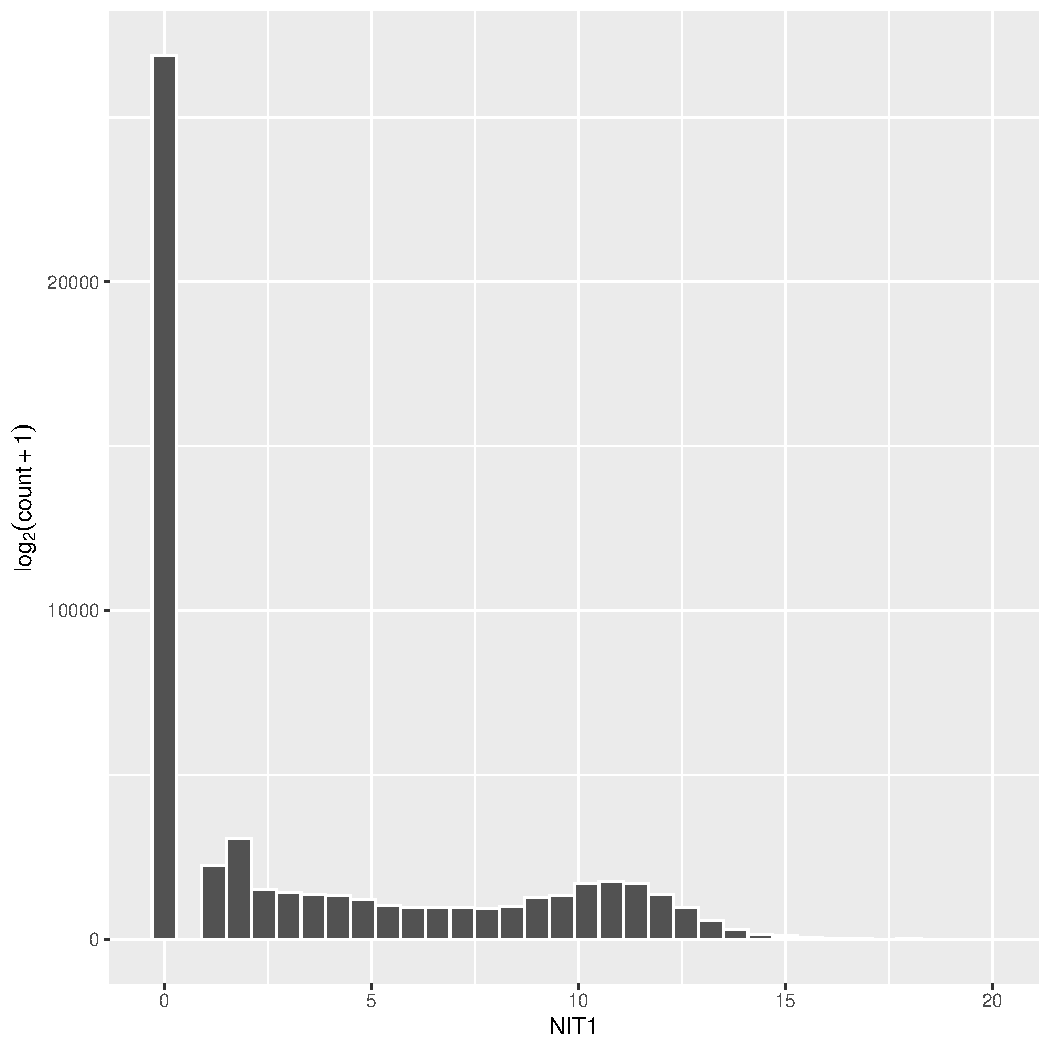
\includegraphics{ortega_rita_ADO_PEC2_files/figure-latex/visual log2 pseudocounts-1.pdf}

Esta transformación logarítmica podría no ser suficiente para evaluar
realmente cómo se distribuyen los datos, ya que los datos procedentes de
RNA-seq no son homocedásticos, sino que su varianza aumenta según
aumenta la media. Intentamos utilizar una función especializada del
paquete \texttt{edgeR} para hacer una transformación de los datos y
comparamos los resultados:

\begin{Shaded}
\begin{Highlighting}[]
\OperatorTok{>}\StringTok{ }\KeywordTok{library}\NormalTok{(edgeR)}
\OperatorTok{>}\StringTok{ }\NormalTok{pseudoCounts2 <-}\StringTok{ }\KeywordTok{cpm}\NormalTok{(mycounts, }\DataTypeTok{prior.count =} \DecValTok{2}\NormalTok{, }\DataTypeTok{log =} \OtherTok{TRUE}\NormalTok{)}
\OperatorTok{>}\StringTok{ }
\ErrorTok{>}\StringTok{ }\KeywordTok{library}\NormalTok{(ggplot2)}
\OperatorTok{>}\StringTok{ }\KeywordTok{ggplot}\NormalTok{(pseudoCounts, }\KeywordTok{aes}\NormalTok{(}\DataTypeTok{x =}\NormalTok{ pseudoCounts2[, }\DecValTok{1}\NormalTok{])) }\OperatorTok{+}\StringTok{ }\KeywordTok{ylab}\NormalTok{(}\StringTok{"CPM"}\NormalTok{) }\OperatorTok{+}\StringTok{ }
\OperatorTok{+}\StringTok{     }\KeywordTok{xlab}\NormalTok{(}\KeywordTok{names}\NormalTok{(mycounts)[}\DecValTok{1}\NormalTok{]) }\OperatorTok{+}\StringTok{ }\KeywordTok{geom_histogram}\NormalTok{(}\DataTypeTok{colour =} \StringTok{"white"}\NormalTok{, }
\OperatorTok{+}\StringTok{     }\DataTypeTok{fill =} \StringTok{"#525252"}\NormalTok{, }\DataTypeTok{binwidth =} \FloatTok{0.6}\NormalTok{)}
\end{Highlighting}
\end{Shaded}

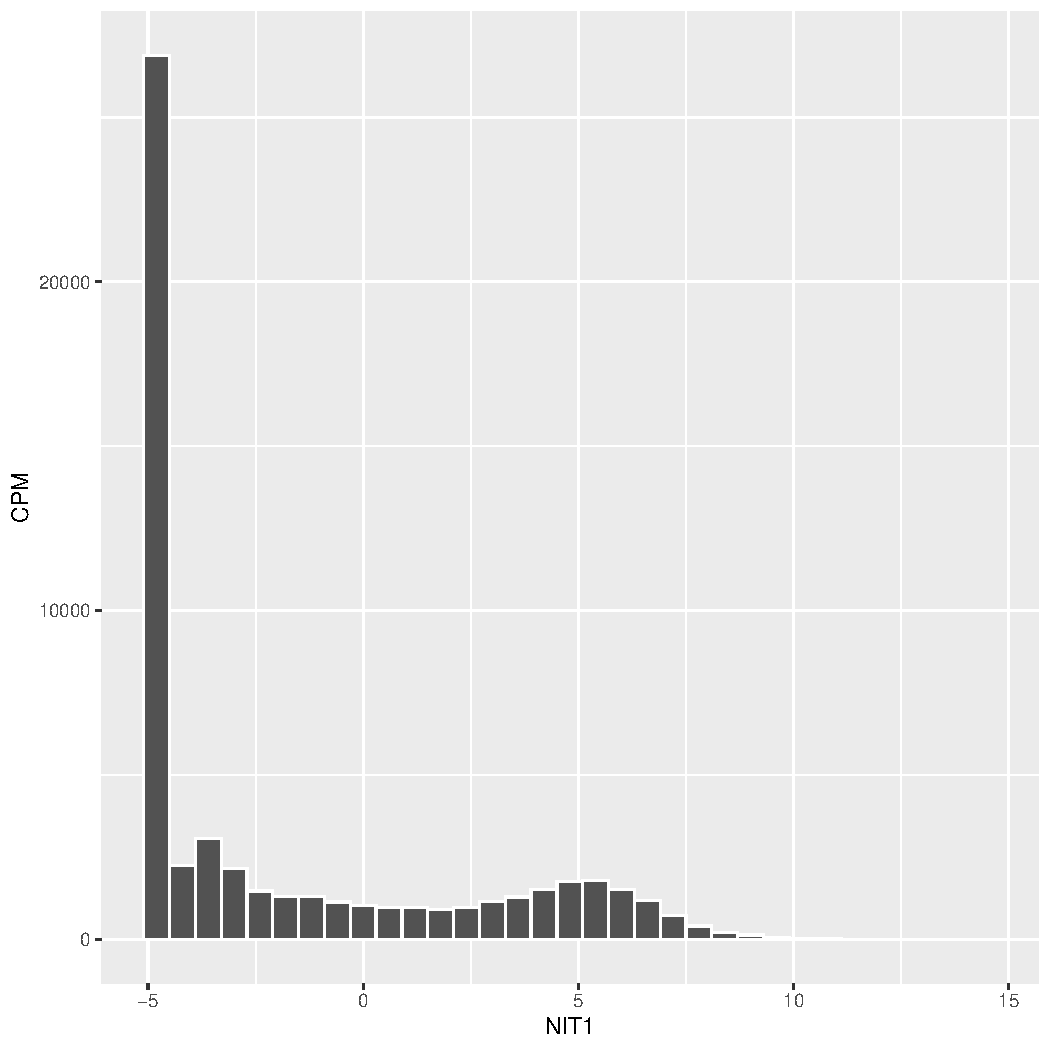
\includegraphics{ortega_rita_ADO_PEC2_files/figure-latex/cpm pseudocount-1.pdf}

Para poder visualizar la distribución de los datos de las 30 muestras
con las que trabajamos, las representamos en forma de boxplot:

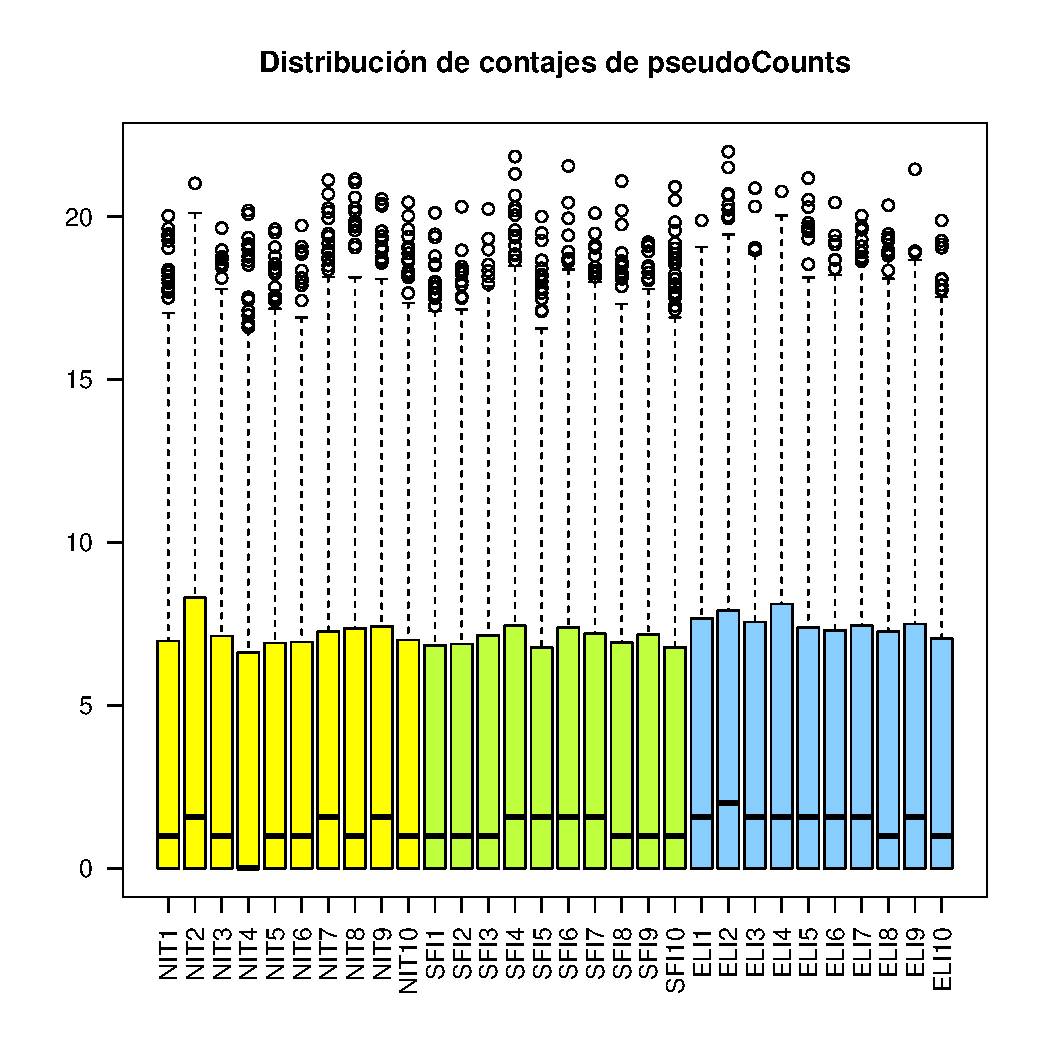
\includegraphics{ortega_rita_ADO_PEC2_files/figure-latex/boxplot_rawdata_pseudocounts-1.pdf}
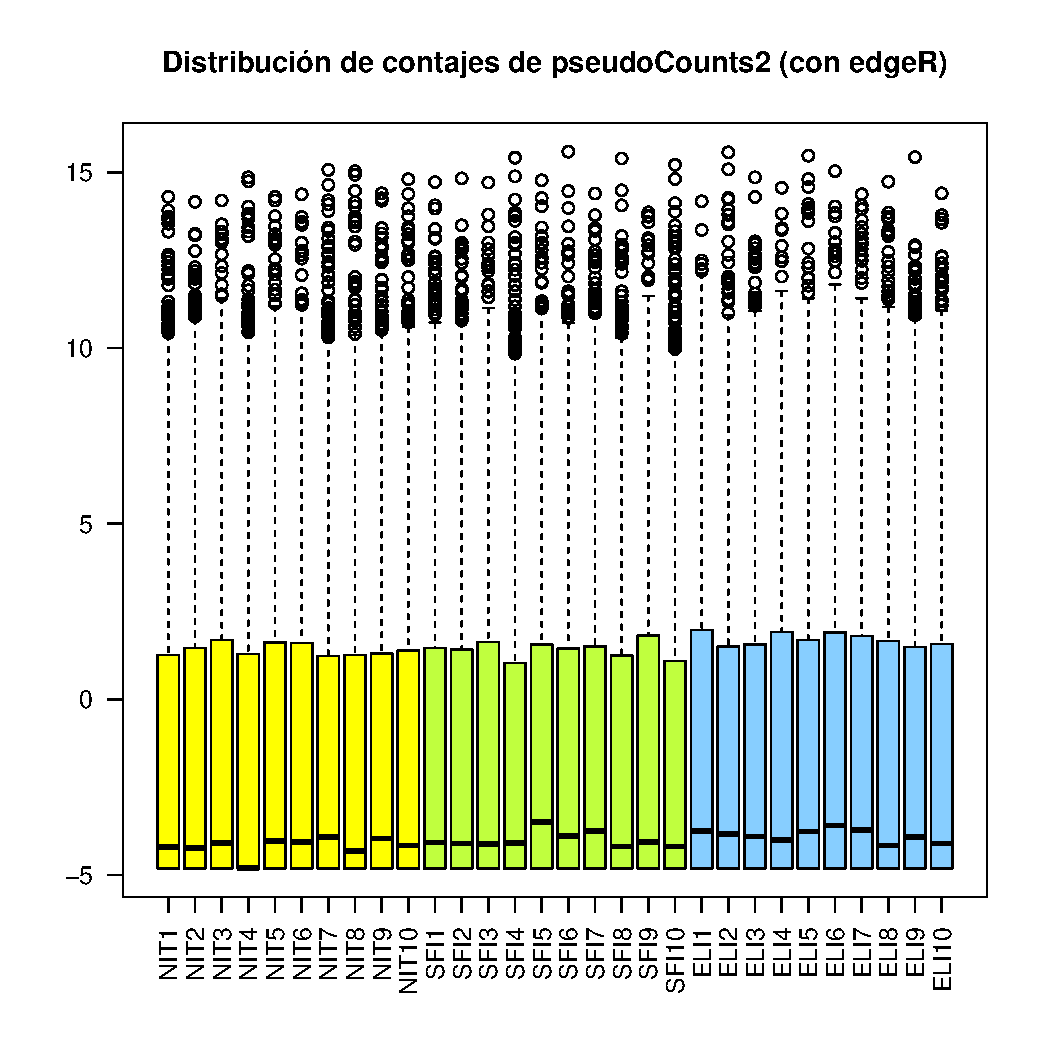
\includegraphics{ortega_rita_ADO_PEC2_files/figure-latex/boxplot_rawdata_pseudocounts2-1.pdf}

Representamos los datos en gráficos de densidades para detectar si
pudiera haber modos secundarios de la distribución de los datos:

\begin{figure}
\centering
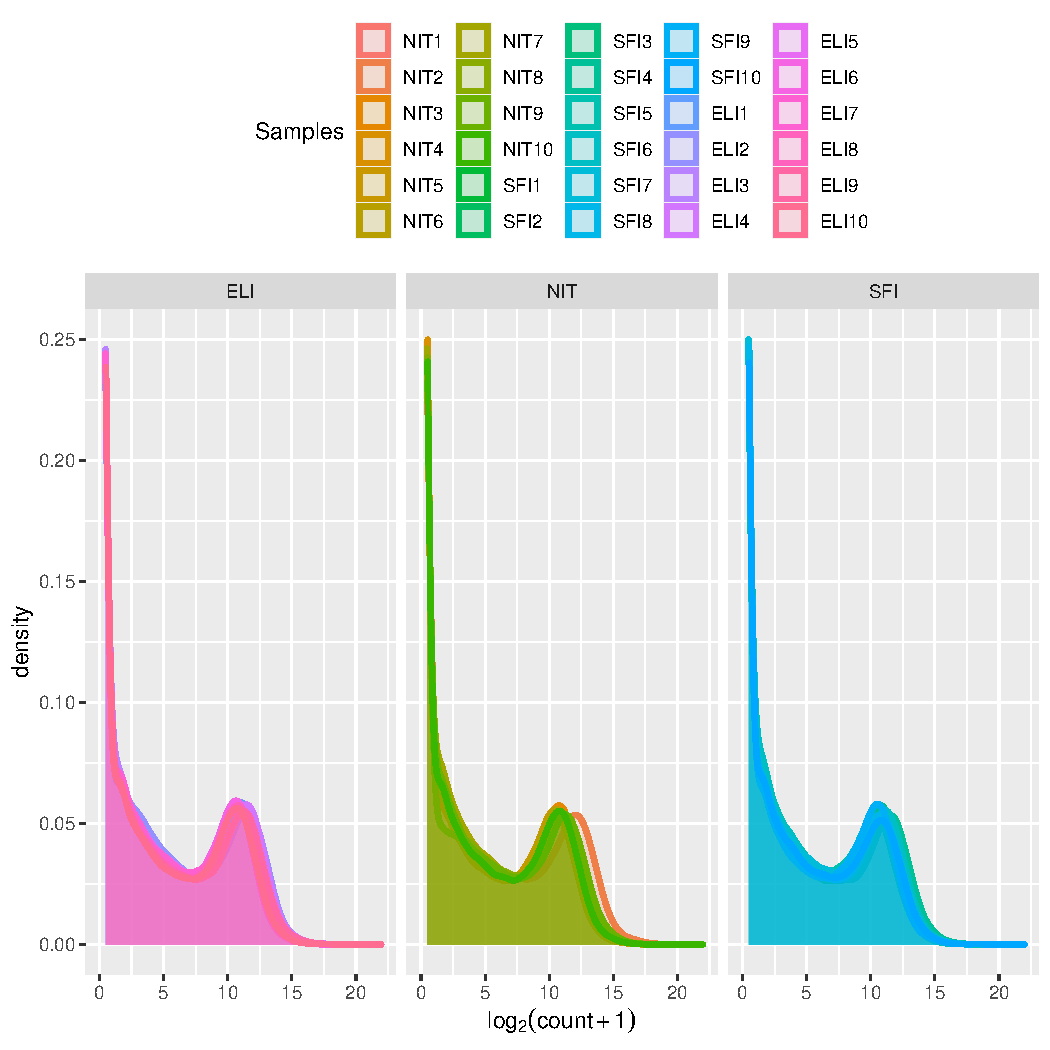
\includegraphics{ortega_rita_ADO_PEC2_files/figure-latex/density_plot-1.pdf}
\caption{Gráficos de densidades que muestra las densidades empíricas de
las muestras individuales dentro de cada una de las tres condiciones
experimentales}
\end{figure}

Para comprobar la reproducibilidad de las muestras, representamos los
MA-plots para comparar muestras entre sí:

\begin{Shaded}
\begin{Highlighting}[]
\OperatorTok{>}\StringTok{ }\NormalTok{myMAplot <-}\StringTok{ }\ControlFlowTok{function}\NormalTok{(dataset, numberX, numberY) \{}
\OperatorTok{+}\StringTok{     }\NormalTok{data <-}\StringTok{ }\NormalTok{dataset}
\OperatorTok{+}\StringTok{     }
\OperatorTok{+}\StringTok{     }\NormalTok{nameX <-}\StringTok{ }\KeywordTok{names}\NormalTok{(data)[numberX]}
\OperatorTok{+}\StringTok{     }\NormalTok{nameY <-}\StringTok{ }\KeywordTok{names}\NormalTok{(data)[numberY]}
\OperatorTok{+}\StringTok{     }
\OperatorTok{+}\StringTok{     }\NormalTok{x <-}\StringTok{ }\NormalTok{data[, numberX]}
\OperatorTok{+}\StringTok{     }\NormalTok{y <-}\StringTok{ }\NormalTok{data[, numberY]}
\OperatorTok{+}\StringTok{     }
\OperatorTok{+}\StringTok{     }\NormalTok{M =}\StringTok{ }\NormalTok{x }\OperatorTok{-}\StringTok{ }\NormalTok{y}
\OperatorTok{+}\StringTok{     }\NormalTok{A =}\StringTok{ }\NormalTok{(x }\OperatorTok{+}\StringTok{ }\NormalTok{y)}\OperatorTok{/}\DecValTok{2}
\OperatorTok{+}\StringTok{     }
\OperatorTok{+}\StringTok{     }\NormalTok{dfMA <-}\StringTok{ }\KeywordTok{data.frame}\NormalTok{(A, M)}
\OperatorTok{+}\StringTok{     }
\OperatorTok{+}\StringTok{     }\KeywordTok{library}\NormalTok{(ggplot2)}
\OperatorTok{+}\StringTok{     }\KeywordTok{ggplot}\NormalTok{(dfMA, }\KeywordTok{aes}\NormalTok{(}\DataTypeTok{x =}\NormalTok{ A, }\DataTypeTok{y =}\NormalTok{ M)) }\OperatorTok{+}\StringTok{ }\KeywordTok{geom_point}\NormalTok{(}\DataTypeTok{size =} \FloatTok{1.5}\NormalTok{, }
\OperatorTok{+}\StringTok{         }\DataTypeTok{alpha =} \DecValTok{1}\OperatorTok{/}\DecValTok{5}\NormalTok{) }\OperatorTok{+}\StringTok{ }\KeywordTok{stat_smooth}\NormalTok{(}\DataTypeTok{se =}\NormalTok{ F, }\DataTypeTok{method =} \StringTok{"loess"}\NormalTok{, }
\OperatorTok{+}\StringTok{         }\DataTypeTok{color =} \StringTok{"red3"}\NormalTok{) }\OperatorTok{+}\StringTok{ }\KeywordTok{ggtitle}\NormalTok{(}\KeywordTok{paste}\NormalTok{(nameX, }\StringTok{" vs "}\NormalTok{, nameY))}
\OperatorTok{+}\StringTok{ }\NormalTok{\}}
\end{Highlighting}
\end{Shaded}

\begin{figure}
\centering
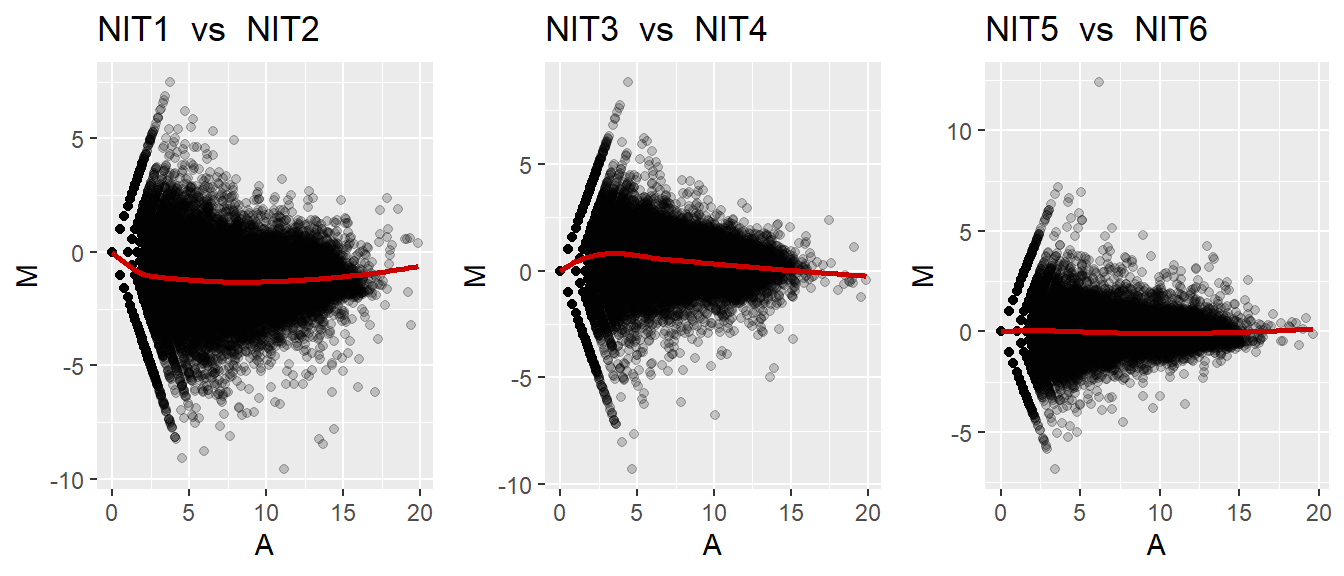
\includegraphics{ortega_rita_ADO_PEC2_files/figure-latex/MAplot_NIT-1.pdf}
\caption{Representación MA de tres comparaciones entre muestras del
grupo NIT}
\end{figure}

\begin{figure}
\centering
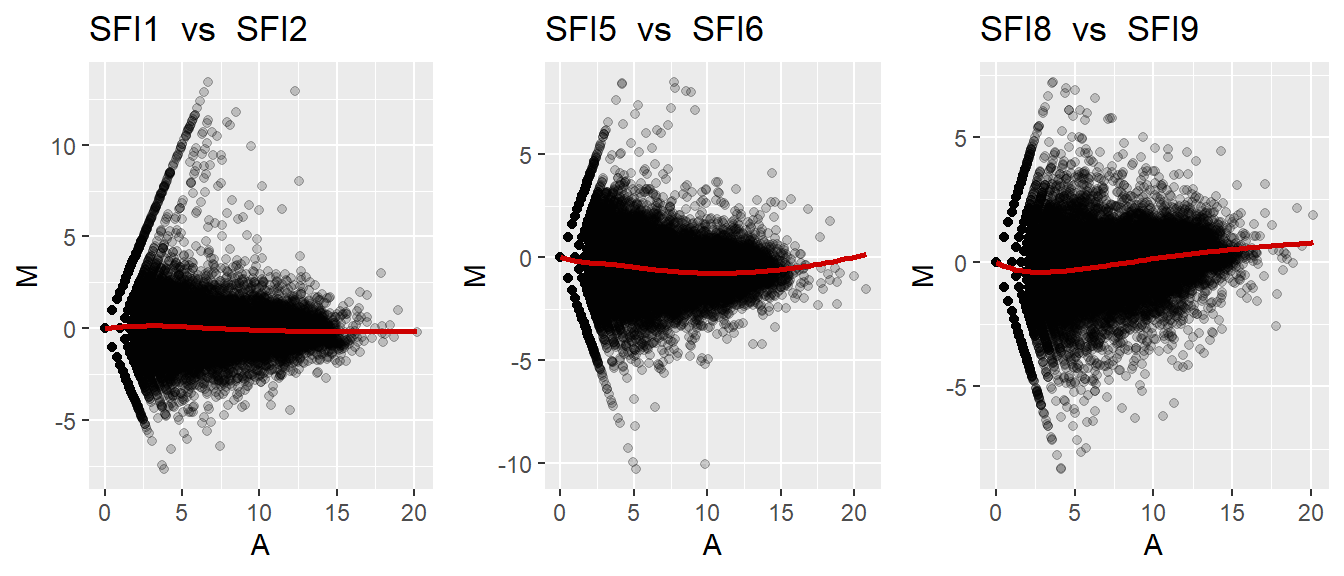
\includegraphics{ortega_rita_ADO_PEC2_files/figure-latex/MAplot_SFI-1.pdf}
\caption{Representación MA de tres comparaciones entre muestras del
grupo SFI}
\end{figure}

\begin{figure}
\centering
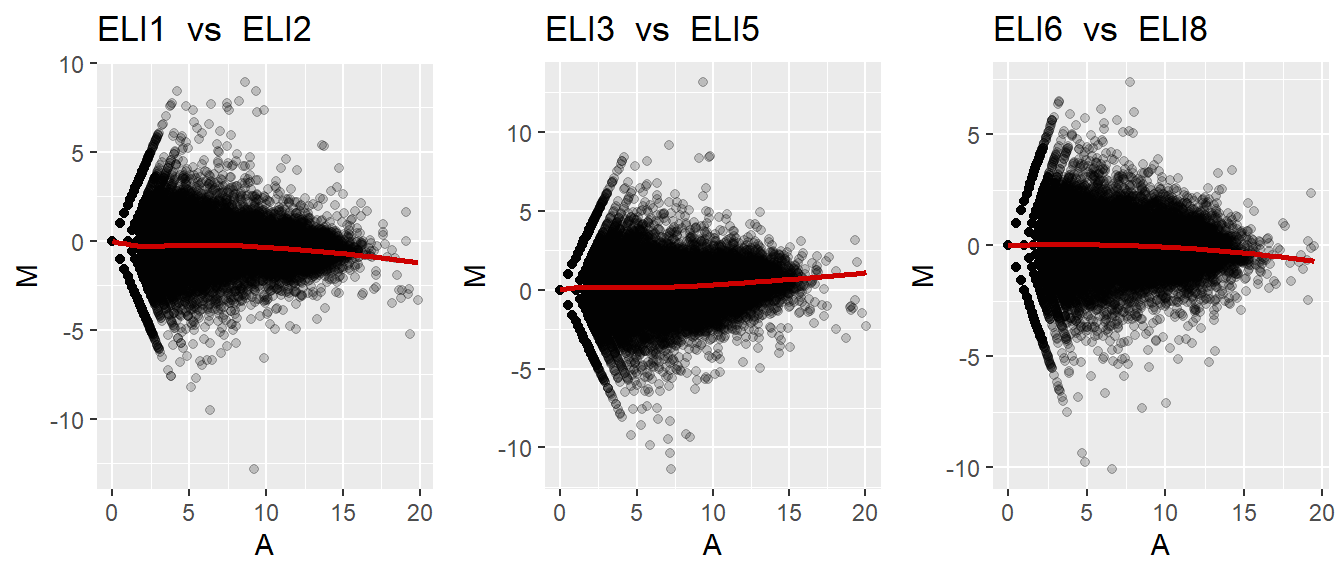
\includegraphics{ortega_rita_ADO_PEC2_files/figure-latex/MAplot_ELI-1.pdf}
\caption{Representación MA de tres comparaciones entre muestras del
grupo ELI}
\end{figure}

Para ver qué muestras son más similares entre sí, las representamos en
un heatmap:

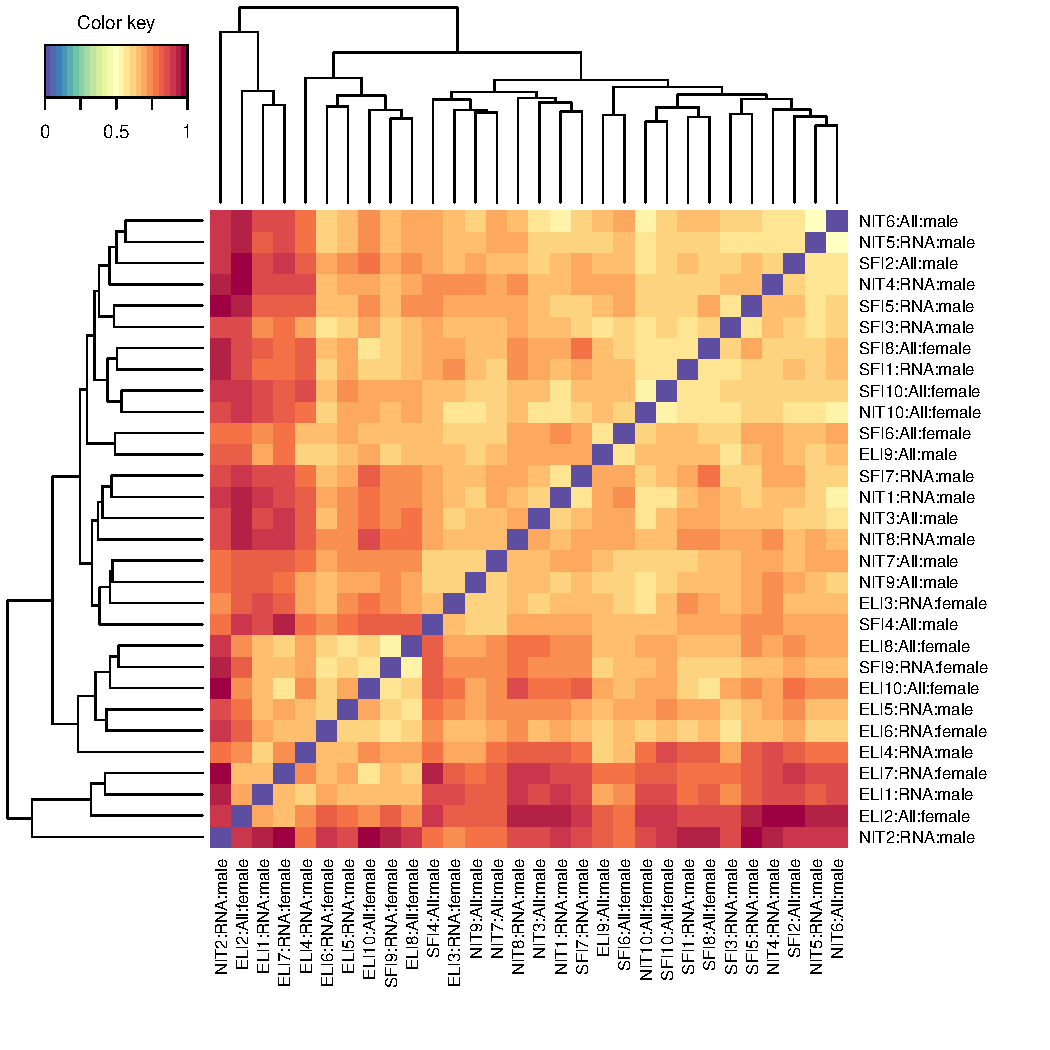
\includegraphics{ortega_rita_ADO_PEC2_files/figure-latex/heatmap_pseudocount-1.pdf}

Mediante un análisis de componentes principales (PCA, \emph{Principal
Component Analysis}), podremos visualizar los efectos de las diferentes
condiciones experimentales y detectar \emph{batch effects}:

\begin{Shaded}
\begin{Highlighting}[]
\OperatorTok{>}\StringTok{ }\KeywordTok{library}\NormalTok{(DESeq)}
\OperatorTok{>}\StringTok{ }\NormalTok{grupo <-}\StringTok{ }\NormalTok{mytargets}\OperatorTok{$}\NormalTok{Group}
\OperatorTok{>}\StringTok{ }\NormalTok{datatype <-}\StringTok{ }\KeywordTok{substr}\NormalTok{(mytargets}\OperatorTok{$}\NormalTok{molecular_data_type, }\DecValTok{1}\NormalTok{, }\DecValTok{3}\NormalTok{)}
\OperatorTok{>}\StringTok{ }\NormalTok{sexo <-}\StringTok{ }\NormalTok{mytargets}\OperatorTok{$}\NormalTok{sex}
\OperatorTok{>}\StringTok{ }\NormalTok{anot <-}\StringTok{ }\KeywordTok{AnnotatedDataFrame}\NormalTok{(}\DataTypeTok{data =} \KeywordTok{data.frame}\NormalTok{(grupo, datatype, }
\OperatorTok{+}\StringTok{     }\NormalTok{sexo, }\DataTypeTok{row.names =} \KeywordTok{colnames}\NormalTok{(pseudoCounts)))}
\OperatorTok{>}\StringTok{ }\NormalTok{exprSetpseudoCounts <-}\StringTok{ }\KeywordTok{new}\NormalTok{(}\StringTok{"ExpressionSet"}\NormalTok{, }\DataTypeTok{exprs =} \KeywordTok{as.matrix}\NormalTok{(pseudoCounts), }
\OperatorTok{+}\StringTok{     }\DataTypeTok{phenoData =}\NormalTok{ anot)}
\end{Highlighting}
\end{Shaded}

\begin{Shaded}
\begin{Highlighting}[]
\OperatorTok{>}\StringTok{ }\KeywordTok{plotPCA}\NormalTok{(exprSetpseudoCounts, }\DataTypeTok{intgroup =} \KeywordTok{c}\NormalTok{(}\StringTok{"grupo"}\NormalTok{, }\StringTok{"datatype"}\NormalTok{))}
\end{Highlighting}
\end{Shaded}

\begin{figure}
\centering
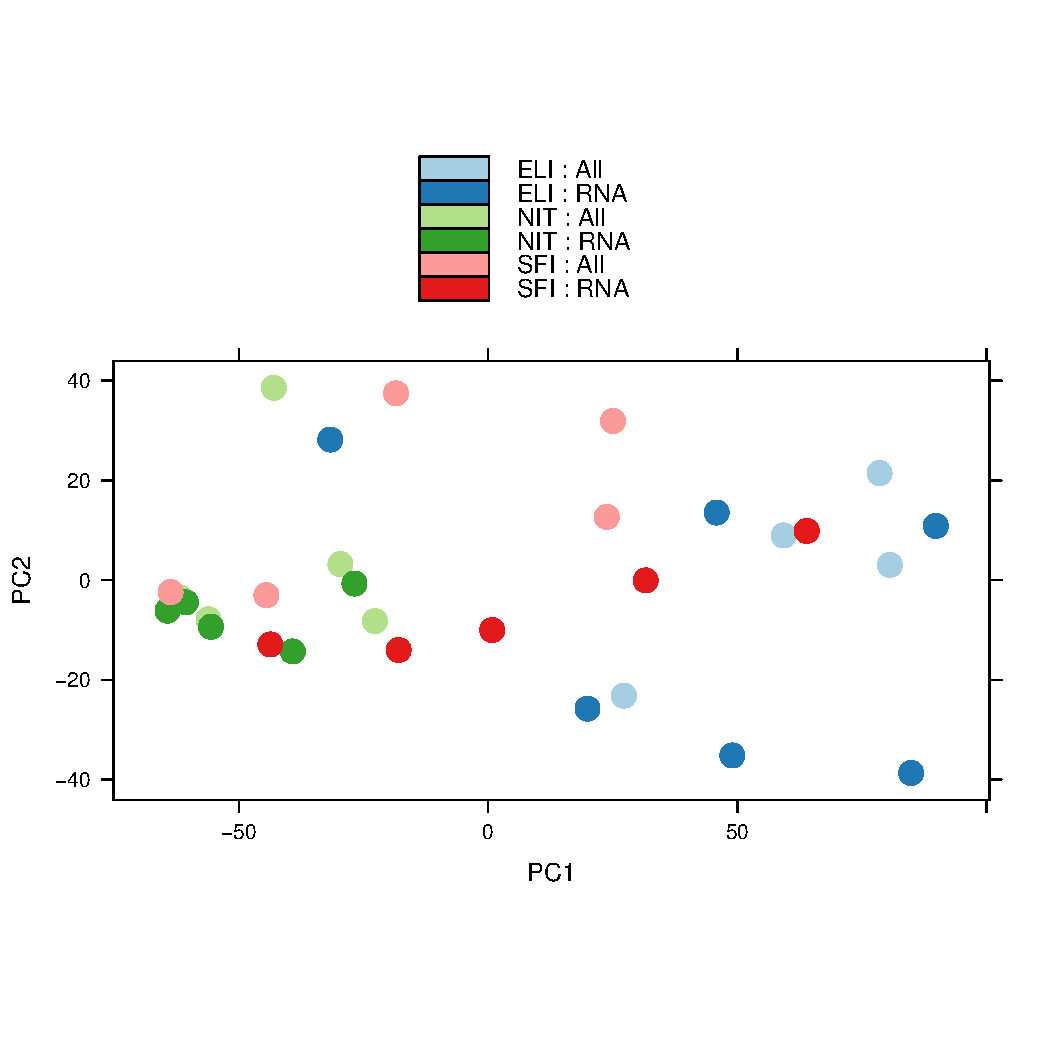
\includegraphics{ortega_rita_ADO_PEC2_files/figure-latex/plotPCA_datatype-1.pdf}
\caption{PCA teniendo en cuenta el grupo experimental y el tipo de
datos}
\end{figure}

\begin{Shaded}
\begin{Highlighting}[]
\OperatorTok{>}\StringTok{ }\KeywordTok{plotPCA}\NormalTok{(exprSetpseudoCounts, }\DataTypeTok{intgroup =} \KeywordTok{c}\NormalTok{(}\StringTok{"grupo"}\NormalTok{, }\StringTok{"sexo"}\NormalTok{))}
\end{Highlighting}
\end{Shaded}

\begin{figure}
\centering
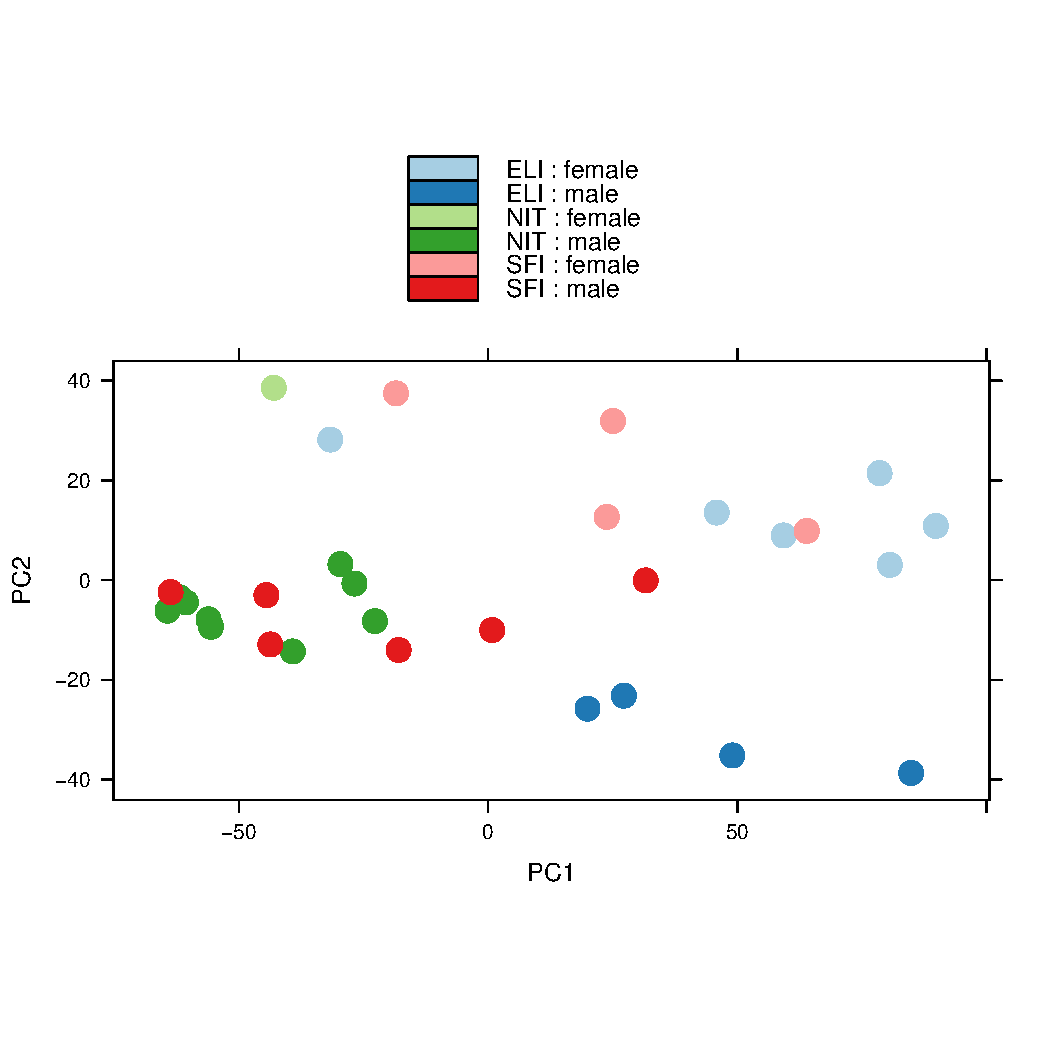
\includegraphics{ortega_rita_ADO_PEC2_files/figure-latex/plotPCA_sexo-1.pdf}
\caption{PCA teniendo en cuenta el grupo experimental y el sexo}
\end{figure}

\hypertarget{filtraje}{%
\subsubsection{Filtraje}\label{filtraje}}

Procedemos a realizar un filtraje de los genes que se ven menos
expresados en todas las condiciones experimentales. Filtramos los genes
que no se expresan en ninguna de las muestras, quedándonos con los que
se expresan al menos en una muestra:

\begin{Shaded}
\begin{Highlighting}[]
\OperatorTok{>}\StringTok{ }\NormalTok{filtro1 <-}\StringTok{ }\KeywordTok{rowSums}\NormalTok{(mycounts) }\OperatorTok{>}\StringTok{ }\DecValTok{0}
\OperatorTok{>}\StringTok{ }\NormalTok{filtro1pseudoCounts <-}\StringTok{ }\NormalTok{pseudoCounts[filtro1, ]}
\OperatorTok{>}\StringTok{ }\KeywordTok{dim}\NormalTok{(mycounts)}
\end{Highlighting}
\end{Shaded}

\begin{verbatim}
[1] 56202    30
\end{verbatim}

\begin{Shaded}
\begin{Highlighting}[]
\OperatorTok{>}\StringTok{ }\KeywordTok{dim}\NormalTok{(filtro1pseudoCounts)}
\end{Highlighting}
\end{Shaded}

\begin{verbatim}
[1] 46229    30
\end{verbatim}

Así hemos reducido el número de genes a
\texttt{nrow(filtro1pseudoCounts)}.

\begin{figure}
\centering
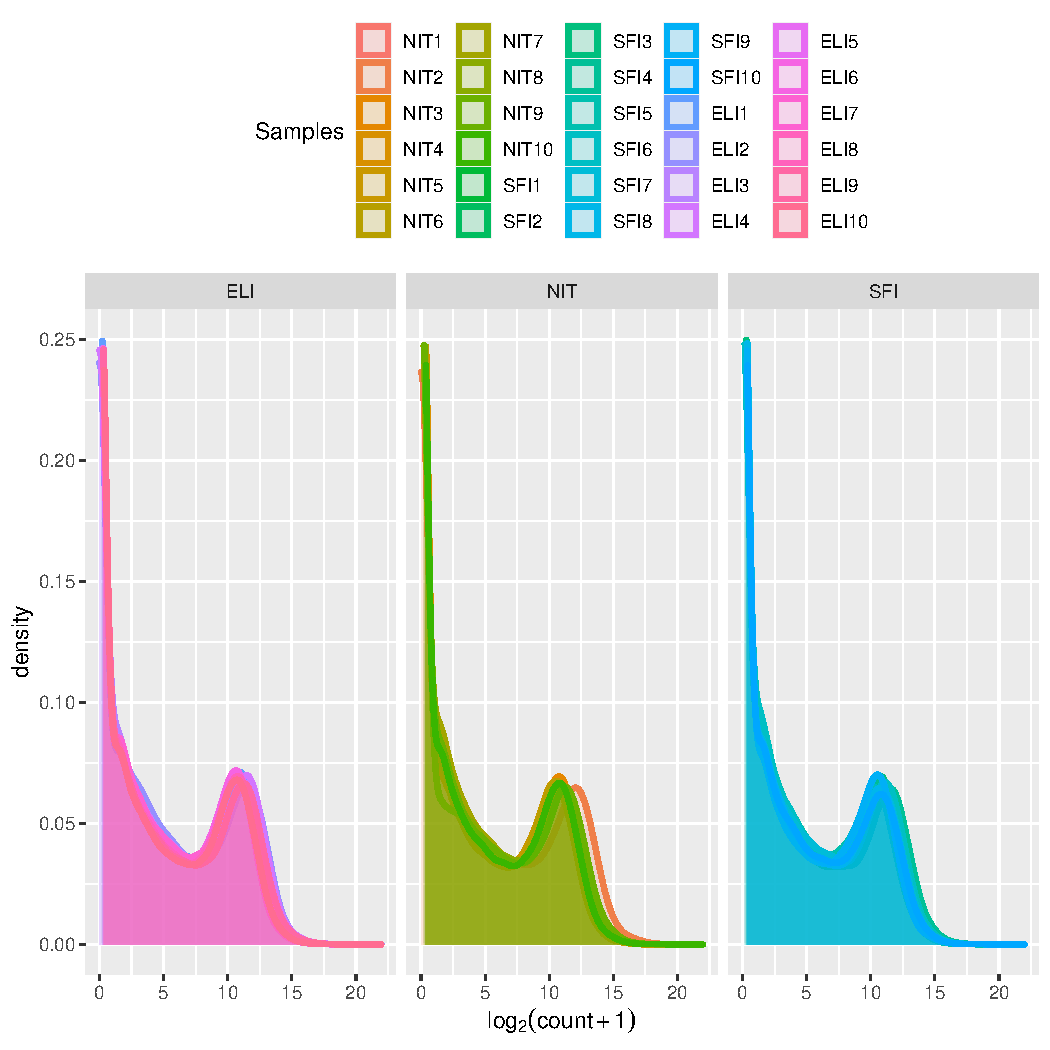
\includegraphics{ortega_rita_ADO_PEC2_files/figure-latex/density_plot_filtro1-1.pdf}
\caption{Diagramas de densidad de las muestras tras el filtrado de los
genes que no se expresan}
\end{figure}

Para poder trabajar con mayor facilidad con los datos, los guardamos
objeto tipo DGElist, con la función \texttt{DGEList} del paquete
\texttt{edgeR}, que nos permite hacer el filtrado de los genes que no se
expresan, tal y como hemos hecho con los \emph{pseudocounts}, pero lo
hacemos de los datos de counts sin la transformación previa que hicimos
para facilitar la representación gráfica:

\begin{Shaded}
\begin{Highlighting}[]
\OperatorTok{>}\StringTok{ }\NormalTok{ConditionDGE <-}\StringTok{ }\NormalTok{mytargets}\OperatorTok{$}\NormalTok{Group}
\OperatorTok{>}\StringTok{ }\NormalTok{DGEFiltered <-}\StringTok{ }\NormalTok{edgeR}\OperatorTok{::}\KeywordTok{DGEList}\NormalTok{(}\DataTypeTok{counts =}\NormalTok{ mycounts, }\DataTypeTok{group =} \KeywordTok{factor}\NormalTok{(ConditionDGE), }
\OperatorTok{+}\StringTok{     }\DataTypeTok{remove.zeros =} \OtherTok{TRUE}\NormalTok{)}
\end{Highlighting}
\end{Shaded}

\hypertarget{normalizaciuxf3n}{%
\subsubsection{Normalización}\label{normalizaciuxf3n}}

Para normalizar nuestros datos, aplicaremos el método \textbf{TMM}
(\emph{Trimmed Mean of M-values}). Al aplicar el TMM, estamos asumiendo
que la mayoría de los genes no están diferencialmente expresados.
Diferentes autores defienden que este método de normalización es
bastante efectivo para detectar genes diferencialmente expresados y para
controlar los falsos positivos (Evans, Hardin, and Stoebel 2017). El
método TMM tiene en cuenta que los pocos genes altamente expresados son
los que más influyen en la expresión total, y que la probabilidad de que
estos genes pueden estar diferencialmente expresados entre muestras en
distintas condiciones, es igual que la probabilidad de que todos los
genes lo estén, es decir, que exista una \emph{expresión balanceada}.
Para aplicar este método de normalización, utilizamos la función
\texttt{calcNormFactors()} del paquete \texttt{edgeR}:

\begin{Shaded}
\begin{Highlighting}[]
\OperatorTok{>}\StringTok{ }\KeywordTok{library}\NormalTok{(edgeR)}
\OperatorTok{>}\StringTok{ }
\ErrorTok{>}\StringTok{ }\NormalTok{NormDGEpFilt <-}\StringTok{ }\KeywordTok{calcNormFactors}\NormalTok{(DGEFiltered, }\DataTypeTok{method =} \StringTok{"TMM"}\NormalTok{)}
\OperatorTok{>}\StringTok{ }\KeywordTok{dim}\NormalTok{(NormDGEpFilt}\OperatorTok{$}\NormalTok{counts)}
\end{Highlighting}
\end{Shaded}

\begin{verbatim}
[1] 46229    30
\end{verbatim}

Representamos los datos normalizados con el método MDS
(\emph{multidimensional scaling}):

\begin{figure}
\centering
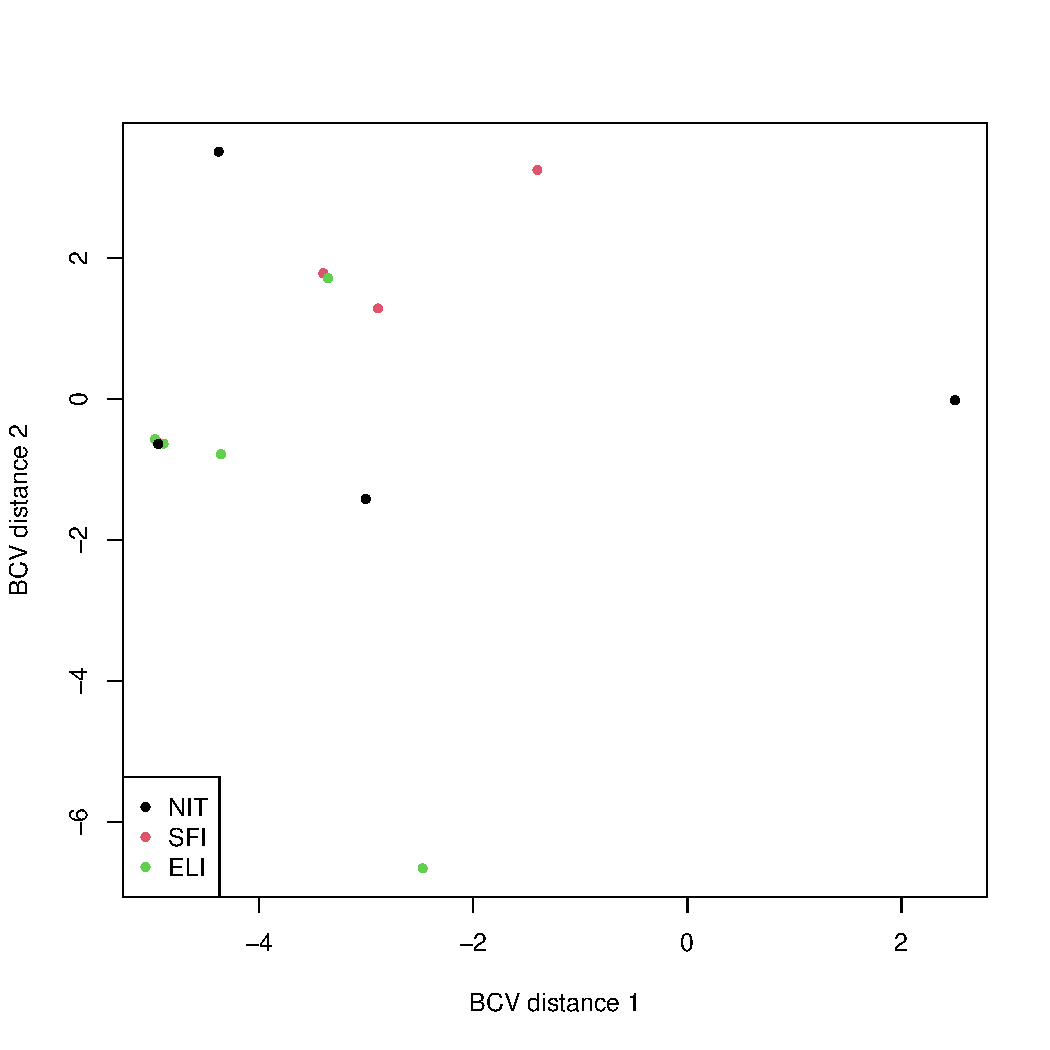
\includegraphics{ortega_rita_ADO_PEC2_files/figure-latex/plot norm_data-1.pdf}
\caption{Representación de los datos normalizados con el método MDS}
\end{figure}

\hypertarget{identificaciuxf3n-de-genes-diferencialmente-expresados}{%
\subsection{Identificación de genes diferencialmente
expresados}\label{identificaciuxf3n-de-genes-diferencialmente-expresados}}

Para identificar los genes diferencialmente expresados entre los
diferentes grupos experimentales, primero debemos estimar el parámetro
de dispersión, que nos indicará el grado de variación dentro de nuestro
dataset.

\begin{Shaded}
\begin{Highlighting}[]
\OperatorTok{>}\StringTok{ }\NormalTok{dispersionComun <-}\StringTok{ }\KeywordTok{estimateCommonDisp}\NormalTok{(NormDGEpFilt, }\DataTypeTok{verbose =}\NormalTok{ T)}
\end{Highlighting}
\end{Shaded}

\begin{verbatim}
Disp = 0.30317 , BCV = 0.5506 
\end{verbatim}

\begin{Shaded}
\begin{Highlighting}[]
\OperatorTok{>}\StringTok{ }\KeywordTok{names}\NormalTok{(dispersionComun)}
\end{Highlighting}
\end{Shaded}

\begin{verbatim}
[1] "counts"            "samples"           "common.dispersion"
[4] "pseudo.counts"     "pseudo.lib.size"   "AveLogCPM"        
\end{verbatim}

A partir de los parámetros de dispersión común calculamos las
dispersiones \emph{Tagwise}:

\begin{Shaded}
\begin{Highlighting}[]
\OperatorTok{>}\StringTok{ }\NormalTok{dispersionComun <-}\StringTok{ }\KeywordTok{estimateTagwiseDisp}\NormalTok{(dispersionComun)}
\OperatorTok{>}\StringTok{ }\KeywordTok{names}\NormalTok{(dispersionComun)}
\end{Highlighting}
\end{Shaded}

\begin{verbatim}
 [1] "counts"             "samples"            "common.dispersion" 
 [4] "pseudo.counts"      "pseudo.lib.size"    "AveLogCPM"         
 [7] "prior.df"           "prior.n"            "tagwise.dispersion"
[10] "span"              
\end{verbatim}

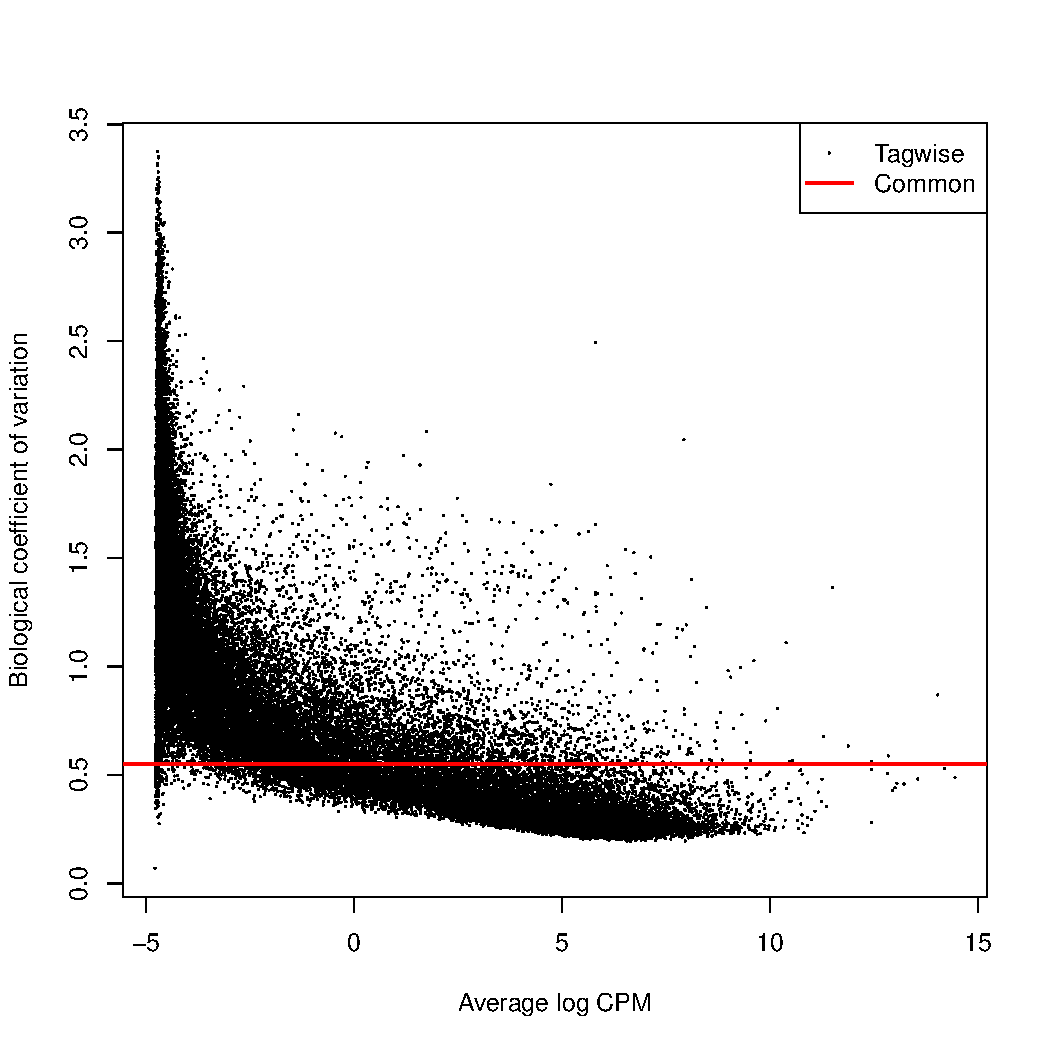
\includegraphics{ortega_rita_ADO_PEC2_files/figure-latex/plotBCV-1.pdf}

\hypertarget{anotaciuxf3n-de-los-resultados}{%
\subsection{Anotación de los
resultados}\label{anotaciuxf3n-de-los-resultados}}

\hypertarget{busca-de-patrones-de-expresiuxf3n-y-agrupaciuxf3n-de-las-muestras-comparaciuxf3n-entre-las-distintas-comparaciones}{%
\subsection{Busca de patrones de expresión y agrupación de las muestras
(comparación entre las distintas
comparaciones)}\label{busca-de-patrones-de-expresiuxf3n-y-agrupaciuxf3n-de-las-muestras-comparaciuxf3n-entre-las-distintas-comparaciones}}

\hypertarget{anuxe1lisis-de-significaciuxf3n-bioluxf3gica-gene-enrichment-analysis}{%
\subsection{\texorpdfstring{Análisis de significación biológica
(``\emph{Gene Enrichment
Analysis}'')}{Análisis de significación biológica (``Gene Enrichment Analysis'')}}\label{anuxe1lisis-de-significaciuxf3n-bioluxf3gica-gene-enrichment-analysis}}

\hypertarget{resultados}{%
\section{Resultados}\label{resultados}}

\hypertarget{discusiuxf3n}{%
\section{Discusión}\label{discusiuxf3n}}

\hypertarget{apuxe9ndice}{%
\section{Apéndice}\label{apuxe9ndice}}

\hypertarget{bibliografuxeda}{%
\section*{Bibliografía}\label{bibliografuxeda}}
\addcontentsline{toc}{section}{Bibliografía}

\hypertarget{refs}{}
\leavevmode\hypertarget{ref-Normalization}{}%
Evans, Ciaran, Johanna Hardin, and Daniel M Stoebel. 2017. ``Selecting
Between-Sample Rna-Seq Normalization Methods from the Perspective of
Their Assumptions.'' \emph{Briefings in Bioinformatics} 19 (5): 776--92.
\url{https://doi.org/10.1093/bib/bbx008}.

\leavevmode\hypertarget{ref-GTEx}{}%
``GTEx Portal.'' n.d. \url{https://www.gtexportal.org/home/}.

\end{document}
